\chapter{Automatic generator}
The automatic generator of Gr\"obner basis solvers is used to easily solve problems leading to systems of polynomial equations. These systems usually arise when solving minimal problems \cite{MinimalProblems} in computer vision. Typically, these systems are not trivial so special solvers have to be designed for concrete problems to achieve efficient and numerically stable solvers. But solvers generated for concrete problems can not be easily applied for similar or new problems and therefore the automatic generator was proposed in \cite{AutoGen}. Solvers generated by the automatic generator can be easily used to solve complex problems even by non-experts users.

The input of the automatic generator is a system of polynomial equations with a finite number of solutions and the output is a MATLAB or a Maple code that computes solutions of the given system for arbitary coefficients. One of the goals of this thesis is to improve previous implementation \cite{AutoGen} of the automatic generator to construct more efficient and numerically stable solvers.

The newest version of the automatic genenerator implemented in MATLAB can be downloaded from \cite{AutomaticGenerator}.

\section{Description of the automatic generator}
In this section we would like to briefly describe the procedure for generating solvers. The procedure is based on computation of the action matrix from which solutions can be obtained. The automatic generator consists of several independent modules, see Figure \ref{autogen:blockDiagram}. Since all these modules are independent, they can be easily improved or replaced by more efficient implementations. Next we describe each of these modules, full description can be found in \cite{AutoGen, KukelovaAlgMethods}.

\begin{figure}[ht]
  \centering
  \includegraphics[width=0.95\textwidth]{AutomaticGenerator.pdf}
  \caption{Block diagram of the automatic generator.}
  \label{autogen:blockDiagram}
\end{figure}

\subsection{Definition of the minimal problem}
\label{subsec:MinimalProblemDefinition}
Definitions of minimal problems to be solved are given in separate functions that are stored in the folder \texttt{minimalProblems}. Each of the definitions has to contain the necessary information about the minimal problem. First of all, the system of polynomial equations with symbolic variables and parameters has to be provided. Next, we have to specify the list of unknown variables and known parameters. Optionally, if we know the monomial basis $B$ of the polynomial system in advance, we can specify it to save some computation time. The monomial basis $B$ is a set $\left\{m\ |\ \overline{m}^G = m\right\}$ where $m$ is a monomial and $G$ is the Gr\"obner basis of the given polynomial system. At last we have to set some settings for the automatic generator. We recommend to obtain the default settings by calling the function \textit{gbs\_InitConfig()} and only overwrite the settings we want to change. In the folder \texttt{minimalProblem}, there are some examples which are self explanatory and can be used as templates to create new minimal problem definitions.

\subsection{Equations parser, instantiating}
In the next step, we have to parse the given equations, which means that we extract monomials and parameters used and obtain total degrees of the polynomials. Then, we instantiate each known parameter with a random number from $\mathbb{Z}_p$. We assign a unique identifier to each parameter used. The reason is that we need to track the parameters through the process of manipulating with the polynomials in order to be able to restore the process in the solver generation module.

\subsection{Monomial basis $B$ computation}
We need to know the monomials basis $B$ to recognize when we have generated all polynomials that are necessary to build the action matrix. If the basis $B$ was not provided within the definition of the minimal problem, we have to compute it. Because there is no function or simple script to compute the basis in MATLAB, we have to do it by calling an external software.

The easiest solution to implement was to use the Maple toolbox for MATLAB. This enables us to call Maple functions from the MATLAB environment directly. To use this option, we have to set \texttt{cfg.GBSolver = @gbs\_findAlgB\_maple} in the settings of the automatic generator. Unfortunately it shows up that the Maple toolbox for MATLAB in not compatible with the MATLAB Symbolic Math Toolbox in versions newer than R2008 so we do not recommend to use this option nowadays but the option is still available on older computers.

The second implemented option is to use the algebraic geometry software Macaulay2 \cite{M2}. In the folder \texttt{gbsMacaulay} there is a template \texttt{code\_template.m2} into which we simply write the given polynomial system. This updated file is saved as \texttt{code.m2} which is executed by Macaulay2 and the results are parsed back in MATLAB. To set up this option, we need to install the software Macaulay2 and set \texttt{cfg.GBSolver = @gbs\_findAlgB\_macaulay} in the automatic generator settings. A problem could be that the Macaulay2 is not easy to set up under the Windows OS. Therefore, the installation file of Macaulay2 is provided within the automatic generator. The only thing that has to be done is to edit the file \texttt{calc.bat} in the folder \texttt{gbsMacaulay} and follow the instructions in the file.

Because of the modularity of the generator, this part can be replaced by another function computing the monomial basis $B$.

The last option is to compute the basis $B$ in advance and set it into the definition of the minimal problem.

In the end, we have to check the number of solutions of the given polynomial system. If there is a finite number of solutions we can continue with the computation.

\subsection{Polynomial generator}
\label{subsec:polynomialGenerator}
To be able to build the action matrix, we have to generate enough polynomials such that after their reduction we get polynomials $q_i$ which have leading monomials from the set $\left(x_k \cdot B\right)\backslash B$ where $x_k$ is a variable and all remaining monomials of $q_i$ are from the set $B$. That is the reason why we had to compute the basis $B$ in the previous step.

In this part of the automatic generator, we represent polynomials as row vectors so that systems of polynomials can be represented by matrices. This representation enables us to easily multiply polynomials with monomials only by shifting the coefficients in the vectors or to reduce the whole polynomial systems by performing the Gauss-Jordan eliminations on the corresponding matrices.

Let $f_i \in F$ where $F$ be a set of polynomials from the input. Let $maxdeg$ be the maximal total degree of all polynomials $f_i$. At the beginning we put all polynomials $\left\{m f_i\ |\ f_i \in F;\ \deg(m f_i) = \deg(f_i),\dots, maxdeg\right\}$ into the matrix $M$, where $m$ is a monomial. Then we perform the Gauss-Jordan elimination on the matrix $M$ and save the result as matrix $\tilde{M}$. Next we check if there exists a variable $x_k$ for which all required polynomials $q_i$ are present in $\tilde{M}$. If we find such a variable, we can continue with the construction of the action matrix for the variable. If not, we have to add more polynomials to the matrix $M$. We increment $maxdeg$ by one and add all polynomials $\left\{m f_i\ |\ f_i \in F;\ \deg(m f_i) = maxdeg\right\}$ to the matrix $M$. Then we continue with the elimination and with the checking the action matrix requirements as explained above. We repeat these steps until all required polynomials $q_i$ are generated so the action matrix can be built. The pseudocode of this process is shown in Algorithm \ref{alg:oneElGen}. The function \textit{CheckActionMatrixConditions} from this code checks if all polynomials $q_i$ are generated in $\tilde{M}$ for at least one variable from the given list of variables. If such a variable is found, the function returns it, otherwise it returns an empty set.

\begin{algorithm}[ht]
  \begin{algorithmic}[1]
    \Require
      \Statex $F$ a set of polynomials
      \Statex $variables$ a list of variables
      \Statex $algB$ a monomial basis $B$
    \Ensure
      \Statex $\tilde{M}$ a matrix representing a set of polynomials
      \Statex $var$ a variable
      \Statex

    \State $maxdeg \gets \max\{\deg(f_i)\ |\ f_i \in F\}$
    \State $M \gets \left\{m f_i\ |\ f_i \in F;\ \deg(m f_i)\ =\ \deg(f_i),\dots,maxdeg;\ m \textrm{ is a monomial} \right\}$
    \State $\tilde{M} \gets$ Reduction to a Row Echelon Form of $M$
    \State $var \gets$ \textit{CheckActionMatrixConditions}$(\tilde{M}, variables, algB)$
    \While{$var = \emptyset$}
      \State $maxdeg \gets maxdeg + 1$
      \State $M \gets M \cup \left\{m f_i\ |\ f_i \in F;\ \deg(m f_i)\ = \ maxdeg;\ m \textrm{ is a monomial}\right\}$
      \State $\tilde{M} \gets$ Reduction to a Row Echelon Form of $M$
      \State $var \gets$ \textit{CheckActionMatrixConditions}$(\tilde{M}, variables, algB)$
    \EndWhile
    \State \Return $(\tilde{M}, var)$
  \end{algorithmic}
  \caption{Polynomial generator -- One elimination solver}
  \label{alg:oneElGen}
\end{algorithm}



In this whole process we need to keep track about how the matrix $M$ was built. Recall that each coefficient of the polynomials $f_i$ has a unique identifier assigned to it in the equations parser. Because the whole matrix $M$ contains only the polynomials $f_i$ or their multiples with monomials, only the coefficients from the polynomials $f_i$ appear in the matrix $M$. We just have to keep the positions of the coefficients. This is done by matrix $\hat{M}$. The matrix $\hat{M}$ is built at the same time as the matrix $M$ by this way. When we put a coefficient into the matrix $M$, we also put the corresponding indentifier to the matrix $\hat{M}$ at the same possition. The matrix $\hat{M}$ enables us to recover the process of polynomial generation in the code generator module.

\subsection{Removing unnecessary polynomials and monomials}
\label{subsec:removingUnPols}
Since the polynomials were generated systematically in the previous step, there may appear some polynomials which are not necessary for the constructing of the action matrix. The goal of this part of the automatic generator is to remove as many polynomials which are not necessary as possible.

We can remove a polynomial $r$ from the matrix $M$ if the corresponding eliminated matrix $\tilde{M}$ still contains all required polynomials $q_i$. In this way we try to remove all polynomials from $M$.

Because the success of removing a polynomial depends on the previous removals, the number of removed polynomials depends on the ordering in which the polynomials are removed. In the automatic generator, we start removing polynomials from the one with the largest leading monomial by monomial ordering used. Because it is very inefficient to remove polynomials one by one and perform each time an expensive Gauss-Jordan elimination, we can enhance the procedure by trying to remove more polynomials at the time. In the automatic generator, this heuristic is used. If we have successfully removed $k$ polynomials, we try to remove $2k$ polynomials in the next step. If the removal of $k$ polynomials have failed, we try to remove $\frac{1}{4}k$ polynomials in the next step. The pseudocode of this removing process is shown as Algorithm \ref{alg:removeUn}.

\begin{algorithm}[!ht]
  \begin{algorithmic}[1]
    \Require
      \Statex $M$ a matrix representing a set of polynomials
      \Statex $variable$ a variable
      \Statex $algB$ a monomial basis $B$
    \Ensure
      \Statex $M$ a matrix representing a set of polynomials
      \Statex

      \State $rows \gets$ number of rows of $M$
      \State $step \gets \max\{\lfloor rows/32\rfloor, 1\}$ 
      \State $up \gets 1$
      \State $filter \gets \{1,2,\dots,rows\}$
      \While{$up \leq rows$}
        \State $down \gets up + step - 1$
	\If{$down > rows$}
          \State $down \gets rows$
	  \State $step \gets down - up + 1$
	\EndIf
	\State $filter_{Old} \gets filter$
	\State $filter \gets filter \backslash \{up, up+1, \dots, down\}$
	\State $\tilde{M} \gets$ Reduction to a Row Echelon Form of $M$ only with rows specified by $filter$
        \State $v \gets$ \textit{CheckActionMatrixConditions}$(\tilde{M}, variable, algB)$
	\If{$v = variable$}
          \State $up \gets down + 1$
	  \State $step \gets 2 step$
	\Else
	  \If{$step = 1$}
	    \State $up \gets up + 1$
	  \Else
            \State $step \gets \max\{\lfloor step/4\rfloor, 1\}$
	  \EndIf
	  \State $filter \gets filter_{Old}$
	\EndIf
      \EndWhile

      \State \Return $M$ only with rows specified by $filter$
  \end{algorithmic}
  \caption{Remove unnecessary polynomials}
  \label{alg:removeUn}
\end{algorithm}



Moreover we can reduce the size of the matrix $M$ by removing unnecessary monomials. A monomial is unnecessary when its removal does not affect the building of the action matrix. We have to keep all monomials such that they are leading monomials of polynominals in the corresponding matrix $\tilde{M}$ and all monomials that are present in the basis $B$. All other monomials can be removed. If we remove all such unnecessary monomials then the matrix $M$ will have dimensions $n \times (n + N)$ where $n$ is the number of the polynomials in the matrix $M$ and $N$ is the number of solutions of the given system.

\subsection{Construction of the action matrix}
This part of the automatic generator starts with the eliminated matrix $\tilde{M}$ of polynomials and variable $x_k$ for which all required polynomials $q_i$ are present in $\tilde{M}$.

Let us describe the construction of the action matrix in an informal and practical way rather than by using the theory. If the theory is needed, it can be found in \cite{KukelovaAlgMethods}. The action matrix $M_{x_k}$ corresponding to the variable $x_k$ is a square matrix of dimensions $N \times N$ where $N$ is the number of elements of the monomial basis $B$. Each row and column of $M_{x_k}$ corresponds to a monomial $b_i \in B$. Let the monomials $b_i$ be sorted such that if $b_l \prec b_k$ then $k < l$ where $\prec$ is the monomial ordering used. We put coefficients of the polynomial $m_i\ =\ \overline{(x_k b_i)}^F$ to the $i$-th row where $F$ are polynomials corresponding to $\tilde{M}$. Because $\tilde{M}$ is in a row echelon form, there are two possibilities how the $i$-th row can be constructed:
\begin{enumerate}
  \item $x_k b_i\ =\ b_j$ for some $b_j \in B$.
	  That means that $x_k b_i$ is irreducible by $F$ and $m_i$ is a monomial in $B$. In this case we set $M_{x_k}(i, j)\ =\ 1$ and $M_{x_k}(i, k)\ =\ 0$ where $k\ \neq\ j$.
  \item $x_k b_i\ \neq\ b_j$ for all $b_j \in B$.
	  In this case there is $f$ such that $\LM(m_i)\ =\ \LM(f)$ where $f \in F$ so $m_i\ =\ x_k b_i - f$. Since all monomials of $f$ except $\LM(f)$ are from $B$, all monomials of $m_i$ are also from $B$. We put coefficient of $m_i$ at the monomial $b_j$ on the $(i, j)$ position in the matrix $M_{x_k}$.
\end{enumerate}

Now, the solutions of the given system can be easily found by computing right eigenvectors of the action matrix $M_{x_k}$.

\subsection{Solver generator}
The last task of the automatic generator is to create a solver which will solve the given polynomial system for an arbitrary set of parameters preserving its structure. The current version of the automatic generator can generate solvers for MATLAB and Maple but new code generators can be easily added. It can be set in the minimal problem definition by setting \texttt{cfg.exportCode} which solvers will be generated. For instance to create both MATLAB and Maple solvers, we set \texttt{cfg.exportCode = \{'matlab' 'maple'\}}.

To create a solver, we have to restore the process of creation of the matrix $M$. This process is saved as the matrix $\hat{M}$ which contains unique identifiers on the positions where the given parameters have to be put. So the matrix $M$ can be built for each given set of parameters. Then the Gauss-Jordan elimination is called on $M$ so we get the matrix $\tilde{M}$. Now the action matrix is built in the same way as above and the solutions are extracted from it. To sum up, the final solver just creates the matrix $M$ by putting parameters to the correct places. After Gauss-Jordan elimination, the action matrix is built by copying some parts of rows of $\tilde{M}$ and then the solutions are extracted by using the eigenvectors of the action matrix.

\subsection{Usage}
The automatic generator is designed to be used even by non-expert users and to be easily expanded or improved.

At first, the script \texttt{setpaths.m} should be executed from the root directory of the automatic generator. This will add all required paths to the MATLAB environment.

Next we have to set up the definition of the minimal problem we want to solve. How the definition have to be specified it is explained in the section \ref{subsec:MinimalProblemDefinition}. All these definitions are stored in the folder \texttt{minimalProblems}. To generate the solver, we call the function \texttt{gbs\_GenerateSolver(MinimalProblem)} where \texttt{MinimalProblem} is the name of the definition of the minimal problem, i.e. the name of the function in the folder \texttt{minimalProblems}. This will generate solvers \texttt{solver\_MinimalProblem.m} for the MATLAB solver and \texttt{solver\_MinimalProblem.txt} for the Maple solver. These solvers are stored in the folder \texttt{solvers}.

For example, let us present generating of a solver for the 6-point focal length problem \cite{6pt}. We have defined this problem as a function \texttt{sw6pt.m} in the folder \texttt{minimalProblems}. By calling the function \texttt{gbs\_GenerateSolver('sw6pt')} we get solvers \texttt{solver\_sw6pt.m} and \texttt{solver\_sw6pt.txt} in the folder \texttt{solvers}.

\section{Improvements}
The bottleneck of the automatic generator is the polynomial generator module. Since the polynomials are generated systematically, the matrices in the resultant solvers are often bigger than necessary which means that the solvers are not efficient. So, many improvements of the automatic generator \cite{AutoGen} can be done. For example, if we want to generate multiple elimination solvers as suggested in \cite{KukelovaAlgMethods}, the polynomial generator module have to be improved or totaly replaced. In the same way, some strategies from other algorithms, for example from the $F_4$ Algorithm \cite{F4}, can be taken over and implemented into the automatic generator. Because we are mostly working with sparse matrices in the automatic generator, Gauss-Jordan elimination for sparse matrices can be implemented to save some computation time.

\subsection{Reimplementation}
The previous implementation \cite{AutoGen} of the automatic generator was implemented in MATLAB R2008. It shows up that new versions of MATLAB are not backward compatible so the automatic generator fails when lauched in some newer version than R2008. Our first task was to reimplement the old implementation into new version of MATLAB. All changes of the code were minor and just on the implementation level.

One important problem was that the Maple Toolbox for MATLAB in not compatible with the MATLAB Symbolic Math Toolbox anymore. One of the options in the monomials basis $B$ module was to use the Maple toolbox to compute the basis $B$. Because of the new incompatibility, this option can no longer be used and the algebraic geometry software Macaulay2 \cite{M2} have to be used instead.

The new version of the automatic generator, as it is desribed in this thesis, is compatible with the version R2015 of MATLAB 64-bit and 32-bit under Windows and Unix operation systems.

\subsection{Multiple elimination solver}
\label{subsec:multipleSolver}
In the section \ref{subsec:polynomialGenerator}, there is desribed a strategy how to generate polynomials for one eliminiation solvers. However, it may be better to create multiple elimination solvers in some cases. A multiple elimination solver is a solver where polynomials are generated systematically by multiplying already generated polynomials by monomials and reduced each time by Gauss-Jordan elimination. So the task of this section is to describe how the polynomial generator of the automatic generator can be improved to be able to generate polynomials for multiple elimination solvers.

To generate polynomials for multiple elimination solvers, we generate all polynomials up to degree $d$ in each step and then, we perform a Gauss-Jordan elimination on them. We increase the degree $d$ when no new polynomials can be generated by multiplying already generated polynomials by some monomials. We stop this process when all polynomials $q_i$ are generated. 

This strategy is very usefull especially when we are generating solvers for systems with many variables. The reason is that increasing the degree $d$ of generated polynomials leads to a large number of new generated polynomials. The number of monomials of degree $d$ in $n$ unknowns is ${d + n - 1 \choose n - 1}$. Therefore, we add $m{d - eqdeg + n - 1 \choose n - 1}$ polynomials in one iteration where $d$ is the total degree of new polynomials, $eqdeg$ is the total degree of given polynomials and $m$ is number of given polynomials. This number grows rapidly when increasing $d$ and $n$ is large. Therefore, we want to hold $d$ as low as possible.

Now, let us look at the process of generating polynomials in more details. The pseudocode is shown as Algorithm \ref{alg:multiElGen}. Let the $maxdeg$ be the maximal total degree of all polynomials from the given system $F$. At the beginning, we put into the matrix $M_1$ all polynomials up to degree $maxdeg$ such that they are product of polynomials from $F$ and some monomials. We get the matrix $\tilde{M}_1$ by eliminating the matrix $M_1$. We check if there exists a variable for which all polynomials $q_i$ are generated in $\tilde{M}_1$. If no such variable is found, we generate new polynomials with higher total degree. We increase the degree $maxdeg$ which is the maximal total degree of all already generated polynomials. The variable $step$ tells how much we want to increase the total degree in one step. We save the $maxdeg + 1$ from the previous iteration into the variable $mindeg$ to keep the track to which degree we have generated polynomials already. We get new matrix $M_2$ by copying the matrix $\tilde{M}_1$ and we add all polynomials with total degrees from $mindeg$ to $maxdeg$ to $M_2$. These polynomials are multiples of polynomials from $\tilde{M}_1$ by some monomials. We save the result of the Gauss-Jordan elimination as the matrix $\tilde{M}_2$. We repeat this process until no new polynomials are added in the iteration. That situation happens when two matrices $\tilde{M}_j$ and $\tilde{M}_{j-1}$ have the same number of non-zero rows. In this case we check if all polynomials $q_i$ are generated for some variable. If not, we have to generate new polynomials with higher total degree. If the variable has been found, we return the last generated matrix $\tilde{M}_j$ and the variable. You may notice that when we are leaving the repeat-until loop on line \ref{alg:multiElGen:rue}, there are two equivalent matrices $\tilde{M}_j$ and $\tilde{M}_{j-1}$. These matrices have the same non-zero rows and differ only by the number of zero rows. This is the reason why we can remove the matrix $\tilde{M}_j$ by decrementing the variable $j$ on line \ref{alg:multiElGen:shred}.

\begin{algorithm}[ht]
  \begin{algorithmic}[1]
    \Require
      \Statex $F$ a set of polynomials
      \Statex $variables$ a list of variables
      \Statex $algB$ a monomial basis $B$
      \Statex $step$ an integer
    \Ensure
      \Statex $\tilde{M}$ a matrix representing a set of polynomials
      \Statex $var$ a variable
      \Statex

      \State $maxdeg \gets \max\{\deg(f_i)\ |\ f_i \in F\}$
      \State $j \gets 1$
      \State $M_1 \gets \left\{m\times f_i\ |\ f_i \in F;\ \deg(m\times f_i)\ =\ \deg(f_i),\dots,maxdeg;\ m \textrm{ is a monomial} \right\}$
      \State $\tilde{M}_1 \gets$ Reduction to a Row Echelon Form of $M_1$
      \State $var \gets Check\ Action\ Matrix\ Conditions(\tilde{M}_1, variables, algB)$
      \While{$var = \emptyset$}
        \State $mindeg \gets maxdeg + 1$
        \State $maxdeg \gets maxdeg + step$
        \Repeat
          \State $j \gets j + 1$
	  \State $M_j \gets \tilde{M}_{j-1}\ \cup\ \Big\{m \times f_i\ |\ f_i \in \tilde{M}_{j-1};$
	  \StatexIndent[4]$\deg(m\times f_i)\ = \ mindeg,\dots,maxdeg;\ m \textrm{ is a monomial}\Big\}$
          \State $\tilde{M}_j \gets$ Reduction to a Row Echelon Form of $M_j$
        \Until{number of nonzero rows of $\tilde{M}_j =$ number of nonzero rows of $\tilde{M}_{j-1}$}\label{alg:multiElGen:rue}
	\State $j \gets j - 1$\label{alg:multiElGen:shred}
        \State $var \gets Check\ Action\ Matrix\ Conditions(\tilde{M}_j, variables, algB)$
      \EndWhile
      \State \Return $(\tilde{M}_j, var)$
  \end{algorithmic}
  \caption{Polynomial generator -- Multiple elimination solver}
  \label{alg:multiElGen}
\end{algorithm}



We have to keep track about how the matrices $M_j$ were built to be able to restore the process of generation of polynomials and generate the code of the solver in the solver generator module. Therefore, we build a matrix $\hat{M}_j$ for each matrix $M_j$. The first matrix $\hat{M}_1$ is built in the same way as the matrix $\hat{M}$ when generating one elimination solver. This matrix contains only the unique identifiers of parameters on positions were real values will be put. Because each matrix $M_j$ is built from the matrix $\tilde{M}_{j-1}$, the matrix $M_j$ contains only coefficients from the matrix $\tilde{M}_{j-1}$. So, when a coefficient from $(m,n)$ position in $\tilde{M}_{j-1}$ is put into $M_j$ at $(k, l)$ position, the tuple $(m, n)$ is put at the position $(k, l)$ of $\hat{M}_j$. So if we have the matrix $\tilde{M}_{j-1}$ and the matrix $\hat{M}_j$, the matrix $M_j$ can be built easily.

To enable generation of multiple elimination solvers, we assign an integer to \texttt{cfg.Poly\-nomials\-Gene\-rator\-Cfg.GJstep} in the settings of the automatic generator. The value of the \texttt{GJstep} has the same meaning as the variable $step$ from the Algorithm \ref{alg:multiElGen}. E.g. by setting \texttt{GJstep = 1} the generated polynomials will be eliminated each time the total degree of generated polynomials is incremented by 1. If we set \texttt{GJstep = 0}, the one elimination solver will be generated as described in the section \ref{subsec:polynomialGenerator}.

\subsection{Removing redundant polynomials}
\label{subsec:removeRedundant}
We may notice that there appear matrices $\tilde{M}_j$ with many zero rows in the process of generation polynomials for multiple elimination solvers. This is because there are many dependent rows in the corresponding matrices $M_j$. These zero rows in matrices $\tilde{M}_j$ give no new information so we want to remove as many as possible rows from the matrices $M_j$ such that the resulting matrices $\tilde{M}_j$ will have the same nonzero rows as before the removal and will have no zero rows.

We know that we can remove the same number of rows from $M_j$ as it is the number of zero rows in $\tilde{M}_j$. But we do not know which rows we should remove. So we try to remove each row $r$ from $M_j$ and if the number of nonzero rows of $\tilde{M}_j$ stays the same, the removal is successful, if not, we have to return the row $r$ back into $M_j$. We end this process of removal when there is no zero row in the matrix $\tilde{M}_j$. Because performing the Gauss-Jordan elimination in each step of removing single row is inefficient we use the same heuristic as desribed in the section \ref{subsec:removingUnPols}. For better understanding, we are providing the pseudocode of this removing as Algorithm \ref{alg:removeRedundant}.

\begin{algorithm}[!ht]
  \begin{algorithmic}[1]
    \Require
      \Statex $M$ a matrix representing a set of polynomials
      \Statex $\tilde{M}$ a matrix in a Row Echelon Form representing a set of polynomials
    \Ensure
      \Statex $M$ a matrix representing a set of polynomials
      \Statex $\tilde{M}$ a matrix in a Row Echelon Form representing a set of polynomials
      \Statex

      \State $toRemove \gets $ number of zero rows of $\tilde{M}$
      \State $nonZero \gets$ number of non zero rows of $\tilde{M}$
      \State $rows \gets$ number of rows of $M$
      \State $step \gets \max\{\lfloor toRemove/4\rfloor, 1\}$ 
      \State $up \gets 1$
      \State $filter \gets \{1,2,\dots,rows\}$
      \While{$toRemove \neq 0$}
        \State $down \gets up + step - 1$
	\If{$down > rows$}
          \State $down \gets rows$
	  \State $step \gets down - up + 1$
	\EndIf
	\State $filter_{Old} \gets filter$
	\State $filter \gets filter \backslash \{up, up+1, \dots, down\}$
	\State $\tilde{M} \gets$ Reduction to a Row Echelon Form of $M$ only with rows specified by $filter$
	\If{number of non zero rows of $\tilde{M} < nonZero$}
          \If{$step = 1$}
	    \State $up \gets up + 1$
	  \Else
            \State $step \gets \max\{\lfloor step/4\rfloor, 1\}$
	  \EndIf
	  \State $filter \gets filter_{Old}$
	\Else
	  \State $toRemove \gets$ number of zero rows of $\tilde{M}$
          \State $up \gets down + 1$
	  \State $step \gets \min\{2 step, toRemove\}$
	\EndIf
      \EndWhile

      \State \Return $(M$ only with rows specified by $filter, \tilde{M})$
  \end{algorithmic}
  \caption{Remove redundant polynomials}
  \label{alg:removeRedundant}
\end{algorithm}



Because this removing process removes only zero rows from the matrices $\tilde{M}_j$ and no others rows are touched it does not influences the process of adding polynomials. Therefore, this removing process is enabled by default and can not be disabled by any option in the automatic generator settings.

\subsection{Matrix partitioning}
\label{subsec:matrixPart}
In the automatic generator, we are dealing with matrices that are mostly sparse, so some efficient techniques can be used to work with them. This will often result in generation of more efficient and numerically stable solvers.

In this section, we focus on how to speed up the Gauss-Jordan elimination of sparse matrices. We use the technique proposed in \cite{SBBD}. We observe that by permuting the rows and the columns of sparse matrices they can be transformed into matrices with block-diagonal structure known as singly-bordered block-diagonal (SBBD) form. Each diagonal block of the SBBD matrices forms an independent problem and therefore, it can be independently eliminated. This speeds up the process of Gauss-Jordan elimination because eliminating more smaller matrices is faster than eliminating one big matrix. If we divide the matrix into $k$ independent blocks that contain comparable number of entries, the speed up is approximately $n^3 \rightarrow k\cdot\big(\frac{n}{k}\big)^3$. Moreover, the permutation matrices that transform matrices to the SBBD forms are precomputed during the solver generation process and therefore, the resultant solver is working already with matrices in the SBBD forms and does not have to spend time by computing the permutation matrices again.

Let us say we want to eliminate matrix $M$. First of all, we have to remove columns that correspond to monomials from the basis $B$ from the matrix because these columns should not be permuted and eliminated. Then, we need to compute the permutation matrix. To compute the permutation matrices, we use the state of the art hypergraph partitioning tool PaToH \cite{PaToH} with settings to divide the matrix into two independent blocks. We do the permutations of rows a columns and get two diagonal blocks $M_{11}$ and $M_{22}$ and coupling columns that can not be assigned to any of the diagonal blocks. Next, we perform two independent eliminations of the blocks $M_{11}$ and $M_{22}$ and permute all rows of $M$ to get the identity matrix in the left top corner. However, we get non-eliminated submatrix in the right bottom corner of $M$. After eliminating this submatrix, the rows above this submatrix are still not eliminated. If this is the last elimination in the solver, we have to eliminate only the rows which we need to build the action matrix from. If this is not the last elimination in the solver, we have to eliminate them all.

\paragraph{Example}
Consider sparse matrix $M$ of size $119\times 143$ as it is shown in Figure \ref{fig:PaToH:start}. Columns 119 -- 143 correspond to monomials from the monomial basis $B$. When we remove these columns, we get a rectangular matrix of size $119 \times 119$ on which we execute the partitioning tool PaToH. After the permutation of the rows and columns, we get the matrix in the SBBD form which can be seen in Figure \ref{fig:PaToH:permutation}. We get two diagonal blocks $M_{11}$ of size $71\times 30$ and $M_{22}$ of size $48 \times 38$ and 51 coupling columns which can not be assigned to any diagonal block. After two independent Gauss-Jordan eliminations of the blocks $M_{11}$ and $M_{22}$ and row permutation, we get the identity matrix in the left top corner, see Figure \ref{fig:PaToH:eliminated}. Now, we have to perform the Gauss-Jordan elimination on submatrix of size $51 \times 75$ in the right bottom corner. After this, we get matrix as it is shown in Figure \ref{fig:PaToH:final}. Now, uneliminated submatrix of size $68 \times 75$ lefts in the right top corner of the matrix. If this is the last elimination in the solver, we do not have to eliminate it whole, but it is sufficient to eliminate only the rows we need to the constructing of the action matrix. If this is not the last elimination in the solver, we have to eliminate the whole remaining uneliminated submatrix.

\begin{figure}[ht]

  \centering
  \begin{subfigure}[b]{0.45\textwidth}
    \centering
    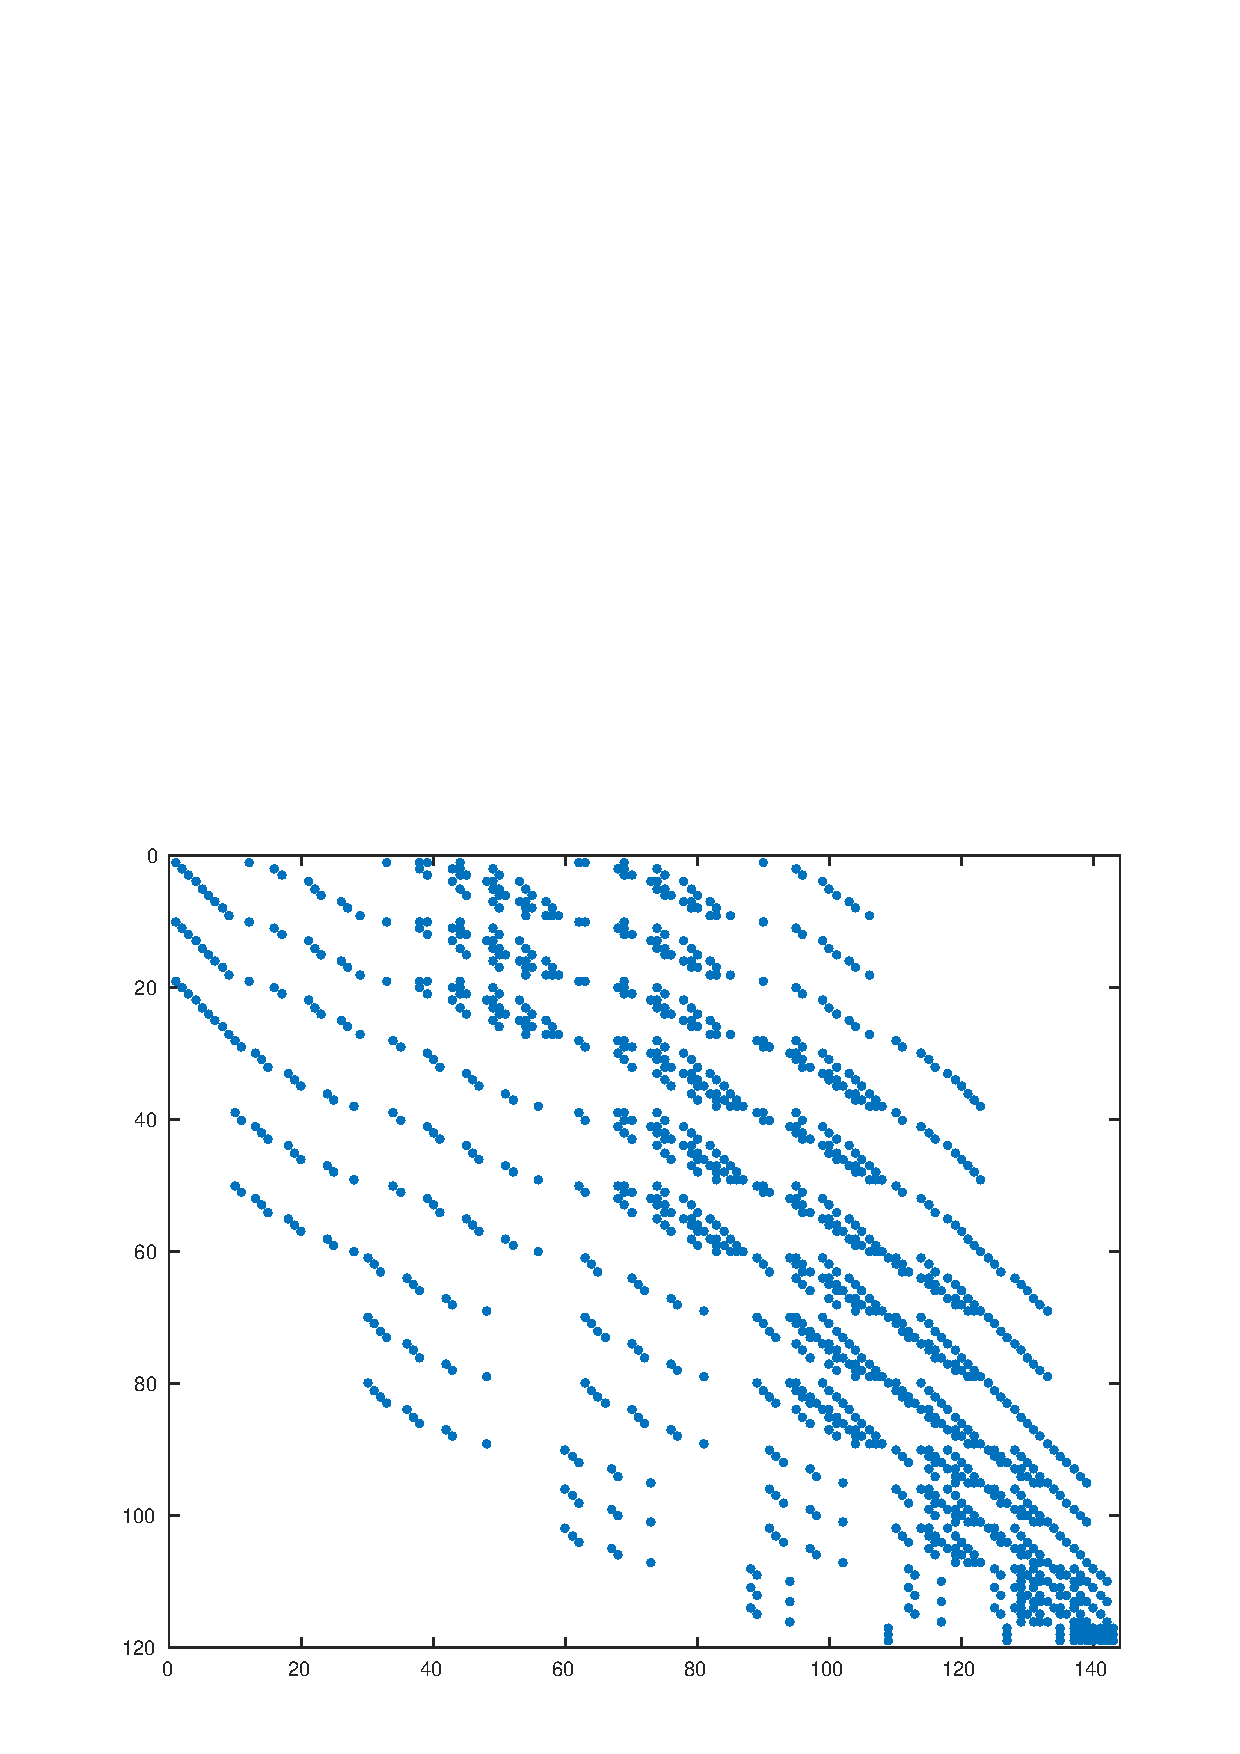
\includegraphics[width=\textwidth]{PaToH/start.pdf}
    \caption{The input matrix.}
    \label{fig:PaToH:start}
  \end{subfigure}
  \hspace{0.5cm}
  \begin{subfigure}[b]{0.45\textwidth}
    \centering
    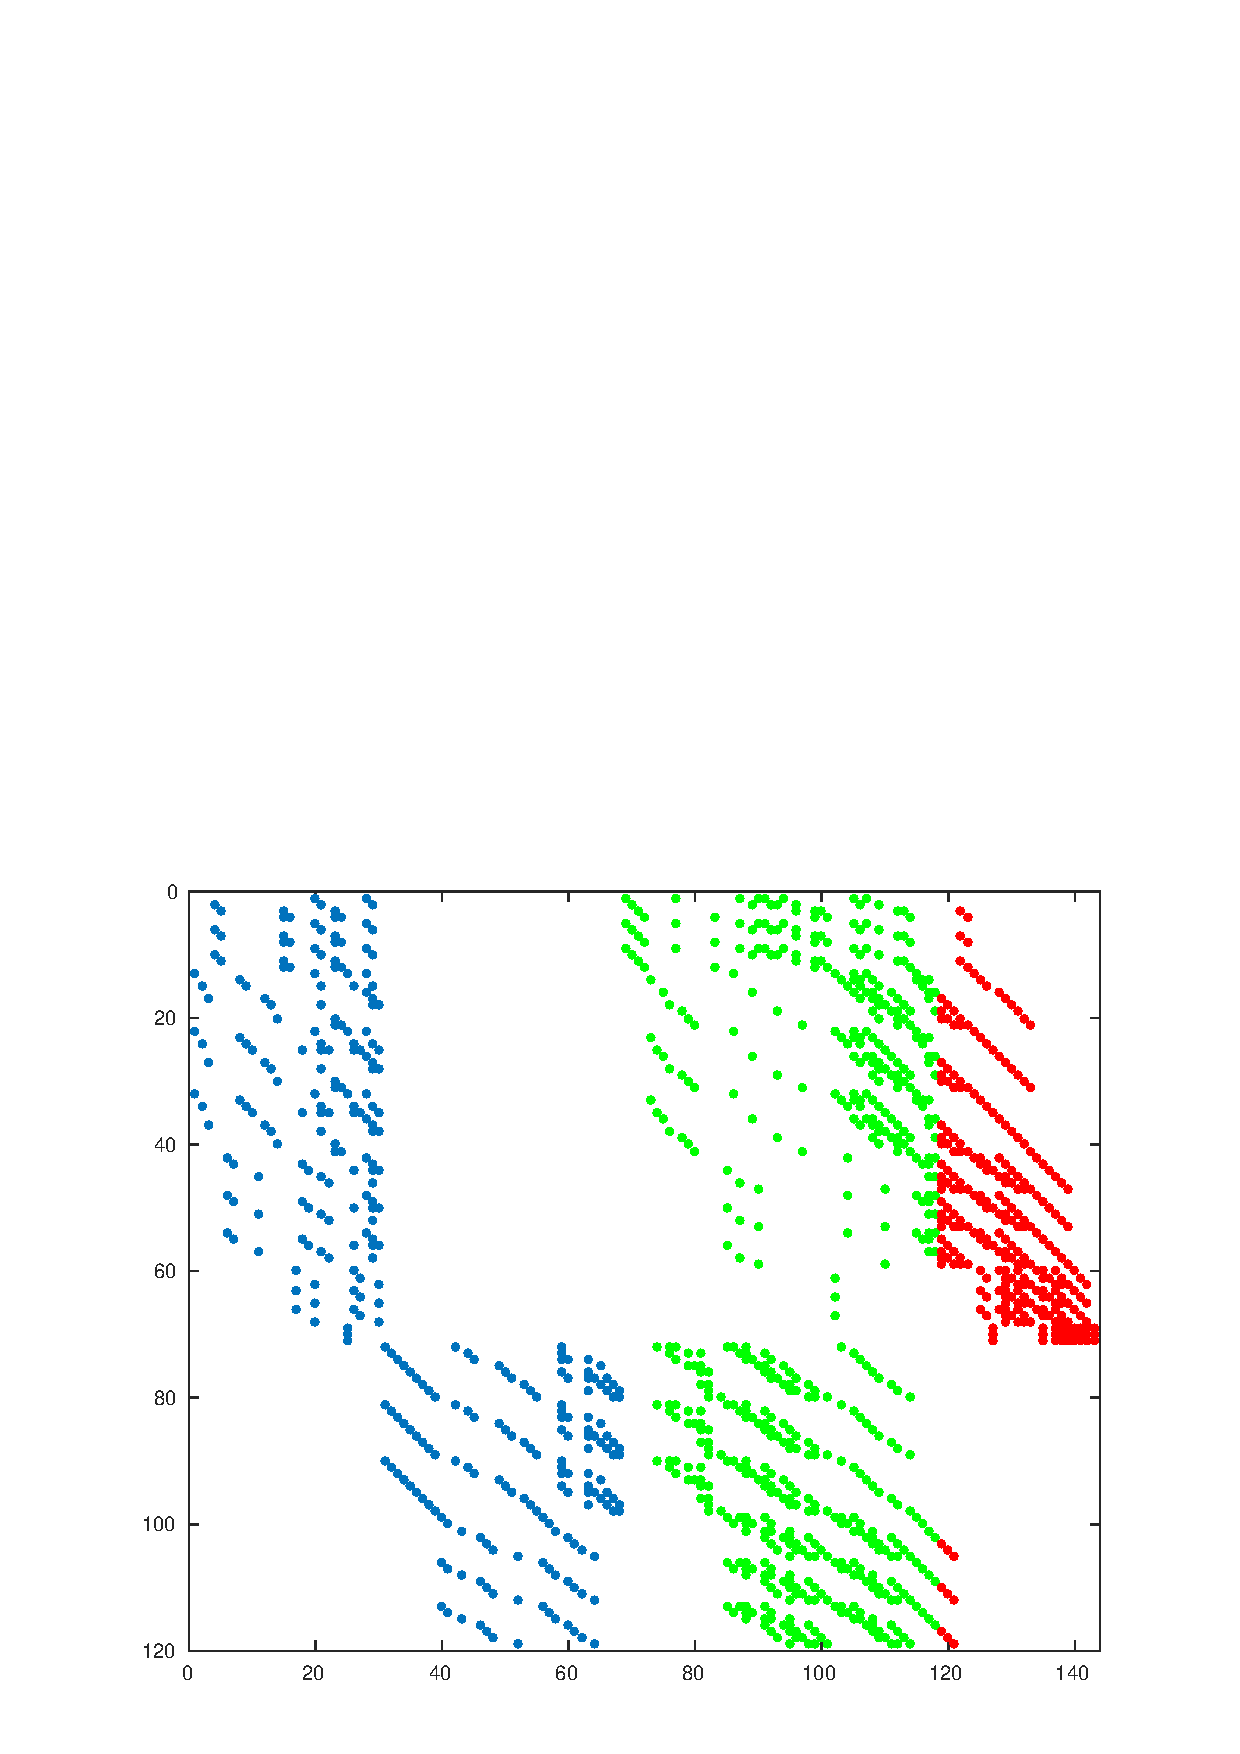
\includegraphics[width=\textwidth]{PaToH/permutation.pdf}
    \caption{The SSBD form of this matrix.}
    \label{fig:PaToH:permutation}
  \end{subfigure}

  \vskip\baselineskip

  \begin{subfigure}[b]{0.45\textwidth}
    \centering
    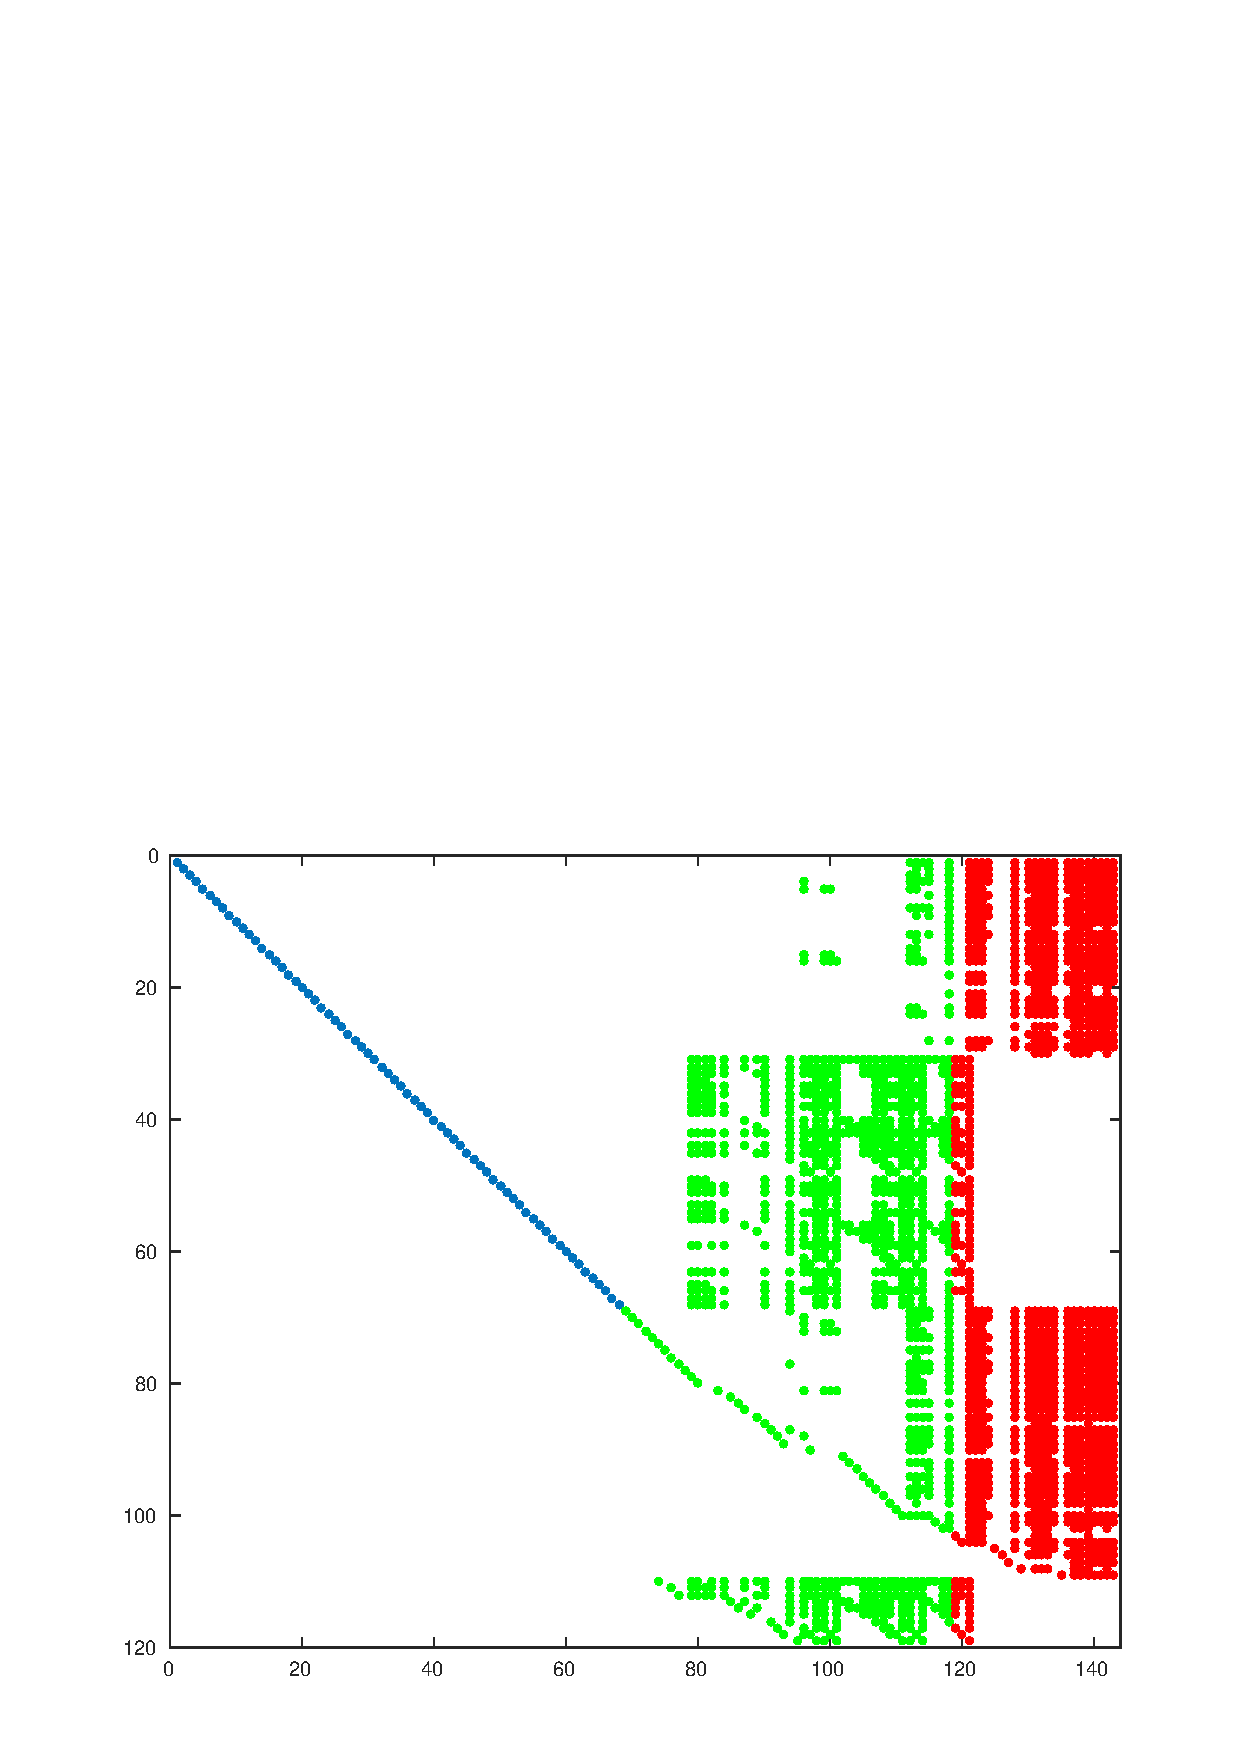
\includegraphics[width=\textwidth]{PaToH/eliminated.pdf}
    \caption{A matrix obtained after two independent Gauss-Jordan eliminations.}
    \label{fig:PaToH:eliminated}
  \end{subfigure}
  \hspace{0.5cm}
  \begin{subfigure}[b]{0.45\textwidth}
    \centering
    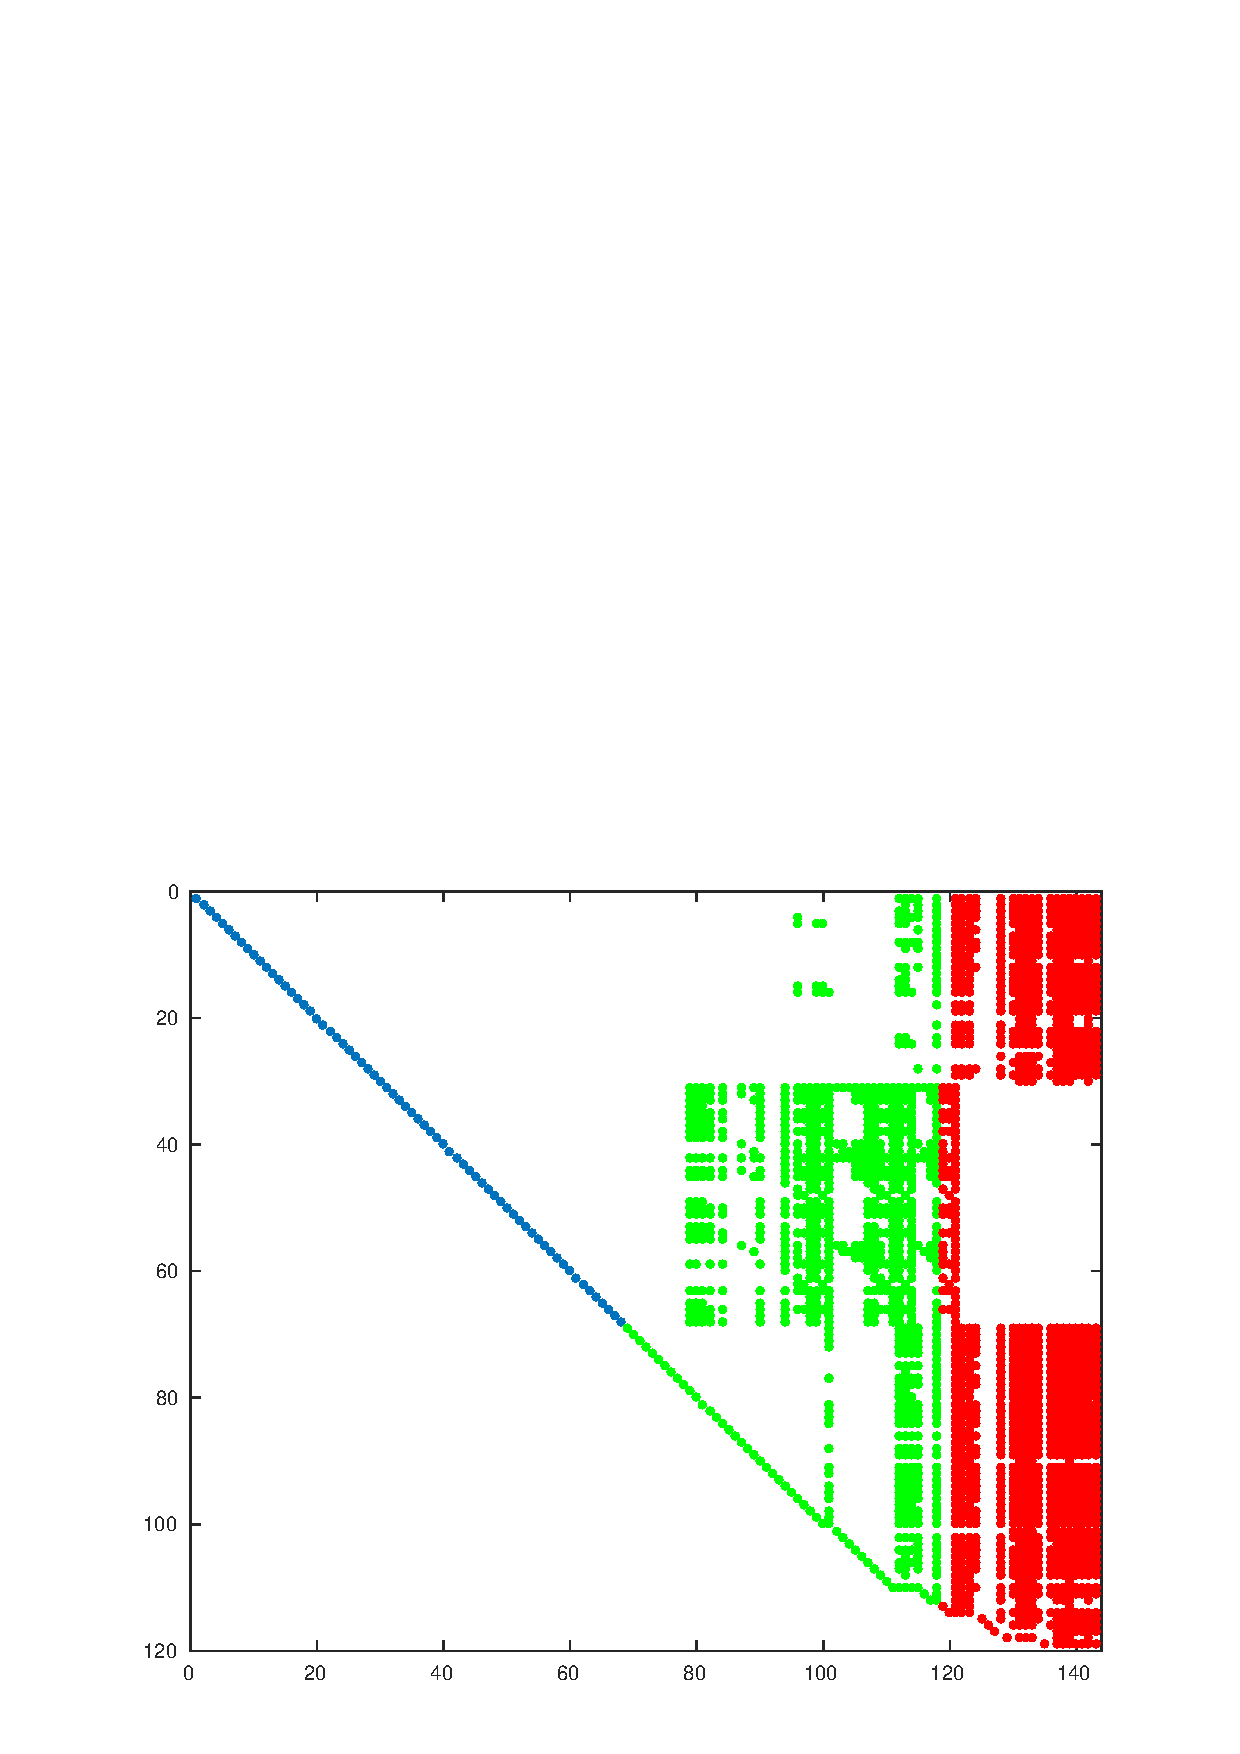
\includegraphics[width=\textwidth]{PaToH/final.pdf}
    \caption{A matrix obtained after elimination of the right bottom submatrix.}
    \label{fig:PaToH:final}
  \end{subfigure}
  \caption{Example of the process of eliminating matrix using matrix partitioning. Colors: blue -- two independent diagonal blocks, green -- coupling columns, red -- columns corresponding to the basis $B$.}

\end{figure}

Since matrix partitioning does not have to be efficient for all minimal problems, it can be easily enabled or disabled in the automatic generator. By setting \texttt{cfg.matrix\-Parti\-tioning = 'all'} matrix partitioning is used to all Gauss-Jordan eliminations in the solver. If \texttt{cfg.matrixPartitioning = 'last'} is set, matrix partitioning is used only to the last Gauss-Jordan elimination in the solver. Matrix partitioning can be totally disabled by setting \texttt{cfg.matrixPartitioning = 'none'}. At last, we want to warn that the tool PaToH is not available under Windows OS so the matrix partitioning can not be used under this system.

\subsection{F4 strategy}
\label{subsec:F4}
Because polynomials are generated systematically in the polynomial generator module, as it is described in section \ref{subsec:polynomialGenerator}, many of them are supefluous and therefore need not be generated. Since the automatic generator consists of independent modules, we can replace the polynomial generator module by some better implementation.

We have described some of the state of the art techniques how polynomial systems can be solved in the chapter \ref{chapter:polynomialSolving}. Therefore, we can take over some of them and implement them into the automatic generator. In the section \ref{sec:F4}, we have understood the $F_4$ \cite{F4} Algorithm so we have implemented this technique into the automatic generator.

\subsubsection{Implementation in Maple}
Before we could start implementing the $F_4$ strategy into the automatic generator, we had to deeply understand the $F_4$ algorithm. Therefore, we have implemented the $F_4$ Algorithm in Maple according to \cite{F4}. 

We have choosen the software Maple because, the $F_4$ Algorithm is implemented there by J. Ch. Faug\`ere himself in the Groebner package. Therefore, we are able to compare our implementation with the implementation by Faug\`ere.

Our implementation of the $F_4$ algorithm is available at \url{http://cmp.felk.cvut.cz/~trutmpav/bachelor-thesis/F4} and it is divided into the same functions as described in \cite{F4}. The Gr\"obner basis generated by the $F_4$ Algorithm are not reduced Gr\"obner basis and therefore, we add the reduction of Gr\"obner basis to get the reduced Gr\"obner basis at the end of the algorithm. This enables us to easily compare the results with results computed by the Faug\`ere's implementation.

The main function is named \textit{F4} in our implementation and it is called \texttt{F4(F, Sel, ordering)} where \texttt{F} is a set of input polynomials, \texttt{Sel} is a function which selects critical pairs as descibed in the section \ref{subsec:F4:sel} and \texttt{ordering} is a monomial ordering. Output of this function is the reduced Gr\"obner basis. Our implementation prints information as the number of pairs, number of selected pairs and their total degree and sizes of matrices during the computation, see an example of the output in Figure \ref{fig:F4:our}. The implementation by Faug\`ere can be called by \texttt{Groebner[Basis](F, ordering, method=fgb)} where the parameters \texttt{F} and \texttt{ordering} have the same meanings as the parameters in our implementation. We can force the Faug\`ere's implementation to print some information about the process by setting \texttt{infolevel[GroebnerBasis] := 5}, see an example of the output in Figure \ref{fig:F4:Faug}. Therefore, we can compare, not only the results, but the sizes of the matrices, too. There are many choices in the $F_4$ Algorithm which can be differently implemented. For example, the list of divisors may be sorted differently in the function \textit{Simplify}. Therefore, the sizes of the matrices may differ in our implementation and in Faug\`ere's implementation, as you can see in the example below.

\paragraph{Example} We show both implementations on the cyclic 4 problem taken from \cite{F4}. You can see the input and the output of our implementation in Figure \ref{fig:F4:our} and of Faug\`ere's implementation in Figure \ref{fig:F4:Faug}.

\begin{figure}[!ht]
  \centering
  \begin{Verbatim}[fontsize=\footnotesize]
> F4([a*b*c*d - 1, a*b*c + a*b*d + a*c*d + b*c*d, a*b + b*c + a*d + c*d, a + b + c + d],
     SelMinDeg, tdeg(a, b, c, d));

        0.00: |P| = 3, Selected 1 of degree 2
        0.00: Symbolic Preprocessing: |L| = 2, |Fd| = 0
        0.01: Reducing matrix of size 3x7
        0.02: Reduction finished

        0.02: |P| = 2, Selected 1 of degree 3
        0.02: Symbolic Preprocessing: |L| = 2, |Fd| = 3
        0.03: Reducing matrix of size 4x9
        0.03: Reduction finished

        0.03: |P| = 2, Selected 2 of degree 4
        0.03: Symbolic Preprocessing: |L| = 4, |Fd| = 7
        0.04: Reducing matrix of size 8x12
        0.05: Reduction finished

        0.05: |P| = 2, Selected 2 of degree 5
        0.05: Symbolic Preprocessing: |L| = 4, |Fd| = 15
        0.06: Reducing matrix of size 6x12
        0.06: Reduction finished

        0.06: |P| = 3, Selected 3 of degree 6
        0.07: Symbolic Preprocessing: |L| = 6, |Fd| = 21
        0.08: Reducing matrix of size 10x14
        0.08: Reduction finished

        0.09: |P| = 2, Selected 2 of degree 7
        0.09: Symbolic Preprocessing: |L| = 4, |Fd| = 31
        0.10: Reducing matrix of size 7x10
        0.10: Reduction finished

        0.10: Computing reduced Groebner basis
\end{Verbatim}
\begin{eqnarray*}
	&  b^2+2bd+d^2\\
	&  a+b+c+d\\
	&  bc^2+c^2d-bd^2-d^3\\
	&  bd^4+d^5-b-d\\
	&  c^3d^2+c^2d^3-c-d\\
	&  d^4c^2+bc-bd+cd-2d^2\\
	&  bcd^2+c^2d^2-bd^3+cd^3-d^4-1
\end{eqnarray*}


  \caption{The input and the output of the cyclic 4 problem using our implementation of the $F_4$ Algorithm in Maple.}
  \label{fig:F4:our}
\end{figure}

\begin{figure}[!ht]
  \centering
  \begin{Verbatim}[fontsize=\footnotesize]
> infolevel[GroebnerBasis] := 5:
> Groebner[Basis]([a*b*c*d - 1, a*b*c + a*b*d + a*c*d + b*c*d, a*b + b*c + a*d + c*d,
                  a + b + c + d], tdeg(a, b, c, d), method=fgb);

-> FGb
 domain: rat_int_cof
 Set offset primes to 0/20000

 Lin Bk ignored [NEW lib]/S:0 -> 8/
 [2](3x7)100%/
 [3](5x10)100%/
 [4](8x12)100%/
 [5](6x12)100%/
 [6](11x16)100%/
 [7](8x11)0.0%/100%/

 Mingbasis2
 (7x24)100%/restore Z1 Copy 80.00 for 24/30 exposants
  {done}
  SWAP Z1/2 Memory usage (estimate):  0.000
   7 polynomials, 30 terms
    total time:         0.014 sec
    ------------------------------
\end{Verbatim}
\begin{eqnarray*}
	&  a+b+c+d\\
	&  b^2+2bd+d^2\\
	&  bc^2+c^2d-bd^2-d^3\\
	&  -1+bcd^2+c^2d^2-bd^3+cd^3-d^4\\
	&  bd^4+d^5-b-d\\
	&  c^3d^2+c^2d^3-c-d\\
	&  d^4c^2+bc-bd+cd-2d^2
\end{eqnarray*}


  \caption{The input and the output of the cyclic 4 problem using Faug\`ere's implementation of the $F_4$ Algorithm in Maple.}
  \label{fig:F4:Faug}
\end{figure}

\subsubsection{Integration into the automatic generator}
Implementation of the $F_4$ Algorithm in the automatic generator is the same as J. Ch. Faug\`ere has described in \cite{F4} and we did in section \ref{sec:F4}. The only difference is that we need to track how the polynomials are constructed to be able to reconstruct the process in the solver generator module. In the $F_4$ Algorithm, to be concrete, in the function \textit{Symbolic Preprocessing}, we are constructing matrices $F_i$ from the selected pairs and polynomials from Gr\"obner basis $G$ that are multiplied by a monomial. Polynomials that are constructed from the selected critical pairs are from $G$ and multiplied by a monomial too. But polynomials in $G$ are just the input polynomials or polynomials from $\tilde{F}_i$ from all previous iterations. All these polynomials that are added into $F_i$ are simplified by the function \textit{Simplify}. That means that such polynomials may be replaced by other polynomials taken from $\tilde{F}_i$. To sum up, the matrix $F_i$ is built from multiples of the input polynomials or polynomials from $\tilde{F}_{1,\dots, i-1}$ and monomials. So to track the process of building the matrices $F_i$, we just have to keep the track of which polynomials from which matrices $\tilde{F}_i$ (we can look at the input polynomials as if it is a matrix $\tilde{F}_0$) are multiplied with which monomials. In the end, we have to recover how the matrix $G$ was build, but this is the same case as reconstructing a matrix $F_i$ because the Gr\"obner basis $G$ consists only of the input polynomials or polynomials from matrices $\tilde{F}_i$.

Unnecessary and redundant polynomials can be, of course, removed from the matrices $F_i$ as we have described in sections \ref{subsec:removingUnPols} and \ref{subsec:removeRedundant}. Moreover, if nothing is added from the matrix $\tilde{F}_i$ to the Gr\"obner basis $G$, i.e. the matrix $\tilde{F}_i^+$ is empty, the matrix $F_i$ can be removed totally. Therefore, there will be no reduction to zero in the generated solver so much computation time can be saved. We are still working with sparse matrices so the matrix partitioning which is described in section \ref{subsec:matrixPart} can be used to speed up the Gauss-Jordan eliminations.

By default, this strategy is disabled in the automatic generator and the systematic polynomial generator as described in sections \ref{subsec:polynomialGenerator} and \ref{subsec:multipleSolver} is used. This is done by setting \texttt{cfg.PolynomialsGenerator = 'systematic'}. To enable the polynomial generator using the $F_4$ strategy, set \texttt{cfg.PolynomialsGenerator = 'F4'} in the automatic generator settings.

The key function in the $F_4$ strategy is the \textit{Sel} function which is descibed in section \ref{subsec:F4:sel}. While different \textit{Sel} functions can be efficient for different minimal problems, it can be easily changed which function will be used. To use the normal strategy, set \texttt{cfg.PolynomialsGeneratorCfg.Sel = @F4\_SelNormal} and to select only one critical pair each time, set \texttt{cfg.PolynomialsGeneratorCfg.Sel = @F4\_SelFirst} in the automatic generator settings. This second function emulates the Buchberger Algorithm. Both this functions are stored in the folder \texttt{generator/F4} and everybody can implement and use his own \textit{Sel} function.

\section{Benchmark}
In the automatic generator as presented in this thesis, there are many different methods which can be used to generate solvers. Efficiency of the generated solvers depends on the method choosen. It shows up that different methods are efficient for different minimal problems. Therefore, we need a tool which will generate more solvers for a choosen minimal problem. Each solver will be generated by a different method used. In the end, the tool will compare the generated solvers so we will be able to choose which solver we will use in applications. The tool have to compare the solver in many aspects because different applications have different requirements. For example, in one application we need solvers which are very fast, in another we may prefere solvers that are slower but more numerically stable. Therefore, we next present such a tool which we call the benchmark of the automatic generator.

\subsection{Structure}
We will briefly describe the structure of the benchmark of the automatic generator. The structure is shown in Figure \ref{autogen:benchmark} and consists of independent blocks which can be easily modified and replaced.

\begin{figure}[ht]
  \centering
  \vspace{0.5cm}
  \includegraphics[height=11cm]{Benchmark.pdf}
  \vspace{0.5cm}
  \caption{Block diagram of the benchmark of the automatic generator.}
  \label{autogen:benchmark}
\end{figure}

At the beginning, we have to load the definition of the minimal problem which we want to generate a solver for. These definitions are described in the section \ref{subsec:MinimalProblemDefinition}.

Next, we load the benchmark templates. A benchmark template is a set of settings of the automatic generator that will be used to generate a solver. For example, if we want to compare one elimination and multiple elimination solvers, we will have two benchmark templates. In the first one, the settings will be set to generate one elimination solver, in the second one, the generation of multiple elimination solver will be set. We store a set of benchmark templates which are related to each other in one MATLAB function. In the example above, we will have both of the templates in one function called \textit{bench\_elimination}. Another example can be, that if we would like to benchmark the polynomial generation methods, i.e. if the $F_4$ method is better than the systematic method, we will have two benchmark templates. The first one will set the automatic generator to generate solvers by the systematical method used. The second one will set the automatic generator to generate solvers by using the $F_4$ strategy. Both this templates will be in one function called \textit{bench\_polynomialGenerator}. We keep all these functions in the folder \texttt{benchmark} in the automatic generator.

When the benchmark templates are loaded, we use the automatic generator to generate the solver for each benchmark template. Then, we run each solver on each instance of parameters and we write down the time spent by the computation. These instances of parameters may be specified by user or if they are not provided, they are randomly generated. The random generator of parameters assign to each parameter random number from the normal distribution with the zero mean and with standard deviation equal to one.

The main part of the benchmark is the evaluation of the results. It is left to the user to implement the evaluation function. This function gets the set of instanced parameters, results from the solver and the correct results, if they are provided with the set of instanced parameters. These correct results may be precomputed in other software only to check the correctness of the results from the generated solvers. The evaluation function returns the set of errors, e.g. how much the results from the solver differ from the correct values. If the evaluation function is not provided by the user, the default evaluation function is used. This function gets the set of given polynomials, substitutes the unknowns by computed solutions and evaluates each polynomial. In the best case, we should get zero for each polynomial. But we obtain non-zero values. Absolute values of these errors depend on the numerical stability of the solver so we are comparing the numerical stability of the generated solvers.

Finally, we have to show the results in some well-arranged way. The presentation of the results is dependent on which data we want to show. Therefore, we leave the implementation of this part to the user. If the user do not specify the function which presents the results, the default presentation function is used. In this function, we get $\log_{10}$ of absolute values of the errors and show them as histogram. To be able to compute the $\log_{10}$ of the errors we have to remove all zero values from the set of errors. We also print the percentage of zero errors amongs all errors.

\subsection{Usage}
The benchmark of the automatic generator is designed to be used easily, but also to be easily modified to give us the results we want to know. The benchmark of minimal problem \texttt{minimalProblem} is called by the command \texttt{gbs\_Benchmark(minimal\-Prob\-lem, bench\-mark, input\-Data, correctOutput, validationFunction, render\-Func\-tion)} where the first two arguments are compulsory and the others are optional. The parameter \texttt{benchmark} is a function handler to the function which provides the set of benchmark templates. The \texttt{input\-Data} is a set of parameters on which we want to test the generated solvers. If this argument is not provided, random generated parameters are used. The \texttt{correctOutput} is a set of expected results of the solvers. These correct outputs are used to compare the numerical stability of the solvers. The function handler \texttt{validationFunction} is a handler to a function which evalutes the results and returns the set of errors. The default \texttt{validationFunction} substitutes computed solutions into the given polynomials and evalutes them. The function handler \texttt{renderFunction} is a handler to a function which shows the results. If this function is not provided, the default function is used. This default function renders histogram of $\log_{10}$ of absolute values of errors.

For clarity, we provide an example. We want to benchmark solvers for the 6-point focal length problem \cite{6pt} and we are considering one elimination and multi elimination solvers. We have no real data to test these solvers and therefore, we have no expected results. We want to use the default validation function and the default function for presenting the results of the benchmark. In this case we call the benchmark with these parameters \texttt{gbs\_Benchmark('sw6pt', @bench\_elimination)}. From the shown results, we decide which solver we will use in the application.
